\subsection{Repaso de clase anterior}
\textbf{Definición de espacio topológico}.

Un \emph{espacio topológico} es un par $(X,\tau)$ donde $X$ es un conjunto y $\tau$ es una colección de subconjuntos de $X$ que verifica:
\begin{enumerate}[]
  \item $\emptyset\in\tau$ y $X\in\tau$;
  \item la intersección de cualquier familia \emph{finita} de
        conjuntos de $\tau$ pertenece a~$\tau$;
  \item la unión de cualquier familia (arbitraria) de conjuntos de
        $\tau$ pertenece a~$\tau$.
\end{enumerate}

\textbf{Definición de continuidad}

Sea $f\colon(X,\mathcal T_1)\to(Y,\mathcal T_2)$. Se dice que $f$ es \emph{continua} si $f^{-1}(V)$ es abierto en $X$ siempre que $V$ es abierto en $Y$.


\textbf{Ejemplo de función NO continua}
Sea
$\operatorname{id}\colon(\mathbb{R}_1,\mathcal T_1)\to(\mathbb{R}_2,\mathcal T_2)$. Observamos que
\[
  \operatorname{id}^{-1}\bigl((0,1)\bigr)=(0,1)\notin\mathcal T_{t},
\]
Por lo que la función identidad $\operatorname{id}$ \emph{no} es continua.

\textbf{Observación:} En general, si $\mathcal T_1$ y $\mathcal T_2$ son topologías sobre un mismo
conjunto~$X$,
\[
  \operatorname{id}\colon(X,\mathcal T_1)\to(X,\mathcal T_2)\text{ es continua}
  \;\Longleftrightarrow\; \mathcal T_2\subseteq\mathcal T_1.
\]

\textbf{Topologías usuales en $\mathbb{R}$}

\subsection{Topologías habituales en $\mathbb{R}$}
\begin{itemize}
  \item Topología usual\; $\mathcal T_{u}$.
  \item Topología discreta\;
        $\displaystyle \mathcal T_{d}=\mathcal{P}(\mathbb{R})$.
  \item Topología trivial\;
        $\displaystyle \mathcal T_{t}=\{\emptyset,\mathbb{R}\}$.
  \item Topología de Zariski\;
        $\displaystyle \mathcal T_{z}=\{A\subseteq\mathbb{R}\mid\mathbb{R}\setminus A
        \text{ es finito}\}$.
  \item Topología co‑numerable\;
        $\displaystyle \mathcal T_{\text{co‑num}}=
        \{A\subseteq\mathbb{R}\mid\mathbb{R}\setminus A
        \text{ es numerable}\}$.
  \item Topología de intervalos semi‑abiertos\;
        $\displaystyle \mathcal T_{ca}=
        \{A\subseteq\mathbb{R}\mid
          \forall x\in A\;\exists a,b:\,[a,b)\subseteq A\}$.
\end{itemize}

\subsection{Interior, Clausura y Puntos Frontera}


\textbf{Nota:} Diremos entonces que $\mathcal T_1$ es \emph{más fina} que $\mathcal T_2$ (o que $\mathcal T_2$ es \emph{más gruesa} que $\mathcal T_1$) cuando $\mathcal T_2\subseteq\mathcal T_1 $ (o $\mathcal T_1\subseteq\mathcal T_2$).

% ----------------------------------------------------------------
%  Conjuntos cerrados
% ----------------------------------------------------------------
\textbf{Definición conjuntos cerrados}
En un espacio topológico $(X,\tau)$, un subconjunto
$A\subseteq X$ es \emph{cerrado} si $X\setminus A$ es abierto.

\textbf{Observación:}
Una topología también puede describirse en términos de sus \emph{cerrados}.
Por ejemplo, la topología de Zariski en~$X$ se obtiene declarando
cerrados los conjuntos finitos de~$X$ y~$X$ mismo:
\[
  \{A\subseteq X\mid A \text{ es finito}\}\cup\{X\}.
\]

% ----------------------------------------------------------------
%  Interior, frontera y clausura
% ----------------------------------------------------------------
Sea $A\subseteq X$ y $x\in X$.  Se presentan tres casos
excluyentes:
\begin{enumerate}[label=(\alph*)]
  \item Existe una vecindad $U$ de $x$ tal que $U\cap A=\varnothing$
        (\emph{punto exterior} de $A$).
  \item Existe una vecindad $U$ de $x$ tal que $U\subseteq A$
        (\emph{punto interior} de $A$).
  \item Para toda vecindad $U$ de $x$ se cumple
        $U\cap A\neq\varnothing$ y
        $U\cap(X\setminus A)\neq\varnothing$
        (\emph{punto de la frontera} de $A$).
\end{enumerate}

\begin{center}
    \shorthandoff{>}
    % --- Solo necesitas \usepackage{tikz} en el preámbulo ---
\begin{tikzpicture}[every node/.style={font=\small}]
    % Conjunto A (elipse roja y sombreado manual)
    \draw[thick,red] (0,0) ellipse (3 and 2);
    % Sombreado: líneas diagonales recortadas por la elipse
    \begin{scope}
      \clip (0,0) ellipse (3 and 2);
      \foreach \x in {-4,-3.6,...,4}
        {\draw[red!60] (\x-3.5,-2.5) -- (\x+3.5,2.5);}
    \end{scope}
    % Etiqueta A
    \node[red] at (1.8,-0.5) {\Large $A$};
  
    % ------------------------------------------------------------------
    % 1. Punto interior (x) y vecindad completamente contenida en A
    % ------------------------------------------------------------------
    \coordinate (xint) at (0.8,0.4);
    \draw[dashed] (xint) circle [radius=0.7];
    \node[blue] at (xint) {\Large $\bullet$};
    \node[blue] at ($(xint)+(0.15,0.55)$) {$x$};
    \node[black] at ($(xint)+(0.95,0.0)$) {$U$};
  
    % ------------------------------------------------------------------
    % 2. Punto exterior (y) y vecindad que no intersecta A
    % ------------------------------------------------------------------
    \coordinate (y) at (-4,1.1);
    \draw[dashed] (y) circle [radius=0.8];
    \node[blue] at (y) {\Large $\bullet$};
    \node[blue] at ($(y)+(-0.1,0.6)$) {$y$};
    \node[black] at ($(y)+(1.05,0.0)$) {$U$};
  
    % ------------------------------------------------------------------
    % 3. Punto de frontera (z) y vecindad que intersecta A y su complemento
    % ------------------------------------------------------------------
    \coordinate (z) at (-1.67,-1.67);
    \draw[dashed] (z) circle [radius=0.8];
    \node[blue] at (z) {\Large $\bullet$};
    \node[blue] at ($(z)+(-0.1,0.6)$) {$z$};
    \node[black] at ($(z)+(1.05,0)$) {$U$};
  \end{tikzpicture}
\shorthandon{>}
\end{center}

Se definen entonces:
\[
  \operatorname{Int}(A)=\{x\in X\mid x \text{ es interior de }A\},\qquad
  \partial A=\{x\in X\mid x \text{ es frontera de }A\},
\]
\[
  \overline{A}= \operatorname{Int}(A)\cup\partial A.
\]

Además
\[
  X=\operatorname{Int}(A)\sqcup\partial A\sqcup
     \operatorname{Int}\!\bigl(X\setminus A\bigr).
\]

\textbf{Ejemplos en la topología usual de $\mathbb{R}$}
\begin{enumerate}
    \item Para los intervalos abiertos:
    \[
  \overline{(a,b)}=[a,b],\qquad
  \operatorname{Int}(a,b)=(a,b),\qquad
  \partial(a,b)=\{a,b\}.
\]
\begin{center}
    \shorthandoff{>}
    \begin{tikzpicture}[>=stealth, every node/.style={font=\small}]
        % Eje real
        \draw[->] (-0.5,0) -- (5.2,0) node[right] {$\mathbb R$};
      
        % Puntos a y b
        \coordinate (a) at (1,0);
        \coordinate (b) at (4,0);
      
        % Interior: segmento grueso entre a y b
        \draw[very thick,blue] (a) -- (b);
      
        % Círculos “abiertos” en a y b  (no pertenecen al interior)
        \draw[line width=1pt,blue,fill=white] (a) circle[radius=3pt];
        \draw[line width=1pt,blue,fill=white] (b) circle[radius=3pt];
      
        % Puntos de la frontera (también son los que faltan para la clausura)
        \draw[fill=red] (a) circle[radius=1.6pt];
        \draw[fill=red] (b) circle[radius=1.6pt];
      
        % Etiquetas
        \node[below] at (a) {$a$};
        \node[below] at (b) {$b$};
        \node[above,blue] at ($(a)!0.5!(b)$) {$\operatorname{Int}(a,b)$};
        \node[above,red]  at (a) {$\partial(a,b)$};
        \node[above,red]  at (b) {$\partial(a,b)$};
      \end{tikzpicture}
    \shorthandon{>}
\end{center}
\item Para los racionales:
\[
  \overline{\mathbb{Q}}=\mathbb{R},\qquad
  \partial\mathbb{Q}=\mathbb{R},\qquad
  \operatorname{Int}(\mathbb{Q})=\varnothing.
\]


\end{enumerate}

% ----------------------------------------------------------------
%  Proposiciones básicas
% ----------------------------------------------------------------
\subsubsection{Propiedades}

Sea $A\subseteq X$. Se verifica que:
\begin{enumerate}[label=\arabic*)]
  \item $\operatorname{Int}(A)$ es abierto.
  \item $\overline{A}$ es cerrado.
  \item $A \overset{\text{ab}} \subseteq X$ es abierto si y sólo si
        $A=\operatorname{Int}(A)$.
  \item $A \overset{\text{cer}} \subseteq X$ es cerrado si y sólo si
        $A=\overline{A}$.
\end{enumerate}

\paragraph{Demostración}
\begin{enumerate}[label=\arabic*)]
  \item Para cada $x\in\operatorname{Int}(A)$ existe una vecindad $U_x\subseteq A$, por lo que si $\{U_x\}_{x\in A}$ es una familia de abiertos, entonces claramente $A=\bigcup_{x\in A}U_x$. Puesto que:
  \begin{itemize}
    \item[$\subseteq$] $A \subseteq \bigcup_{x\in A}U_x$, pues $A \in \{U_x\}_{x\in A}$;
    \item[$\supseteq$] $\bigcup_{x\in A}U_x \subseteq A$, pues $U_x \subseteq A$ para todo $x\in A$.
  \end{itemize}
  \item Dado que sabemos:
  \begin{align*}
      X&=\operatorname{int}{(A)}\sqcup \partial A \sqcup \operatorname{Int}(X\setminus A),\\
      &=\overline A \sqcup \operatorname{Int}(X\setminus A).
  \end{align*}
  y por el inciso 1 $X-\overline A = \operatorname{Int}(X\setminus A) \overset{\text{ab}}\subseteq X$ es abierto, por lo que $\overline A$ es cerrado, por definición.
  \item 
    \begin{itemize}
        \item[$\implies$] Probamos las dos contenencias:
        
        \begin{itemize}
            \item[$\supseteq$] Si $x\in \operatorname{namet}(A)$, entonces existe una vecindad $U$ de $x$ tal que $U \subseteq A$. Luego $\operatorname{Int}(A) \supseteq A$.
            \item[$\subseteq$] Si $x\in A$, entonces $A$ es vecindad de $x$ y por lo tanto $x\in \operatorname{Int}(A)$. Luego $A \subseteq \operatorname{Int}(A)$.
        \end{itemize}
        \item[$\impliedby$] Si $A = \operatorname{Int}(A)$, entonces $A$ es abierto por el inciso 1.
    \end{itemize}
    \item Ejercicio!
\end{enumerate}

% ----------------------------------------------------------------
%  Ejercicios sugeridos
% ----------------------------------------------------------------
\subsection{Ejercicios}
\begin{itemize}
  \item \textit{Hatchet}, pág.\,14--15: \;ej.\;1,2, 4, 5, 6.
  \item \textit{Viro, Ivanov}, pág.\,11: \;2.1, 2.3, 2.6, 2$'$12x, 2.M$_x$.
\end{itemize}

% ----------------------------------------------------------------
%  Bases para una topología
% ----------------------------------------------------------------
\subsection{Bases para una topología}

\textbf{Definición de base.}
Una familia $\mathcal{B}$ de abiertos en $X$ es una \emph{base} si todo abierto de~$X$ puede escribirse como unión de elementos de $\mathcal{B}$.

\paragraph{Ejemplos.}
\begin{enumerate}
  \item $\mathcal{B}=\bigl\{\{x\}\mid x\in X\bigr\}$ es base de la
        topología discreta.
  \item $\mathcal{B}=\bigl\{(a,b)\mid a,b\in\mathbb{R}\bigr\}$ es base
        de la topología usual de $\mathbb{R}$.
  \item $\mathcal{B}'=\bigl\{(a,b)\mid a,b\in\mathbb{Q}\bigr\}$ es base
        de la topología usual de $\mathbb{R}$.
  \item En $\mathbb{R}^2$ con la topología usual:
  \begin{enumerate}[label=\alph*)]
    \item  \( \mathcal{B}_1 =  \{ B_\epsilon^{usual}(\vec{x}) \ | \ \vec{x} \in \mathbb{R}^2, \ \epsilon >0 \} \) es una \textbf{base} (asociada a la \textbf{metrica euclidea} \( l_2 \)). 
    \item \( \mathcal{B}_2 =  \{ B_\epsilon^{inf}(\vec{x}) \ | \ \vec{x} \in \mathbb{R}^2, \ \epsilon >0 \} \) es una \textbf{base} (asociada a la \textbf{metrica euclidea} \( l_\infty \)), muy util en el curso de \textbf{Integracion y Series}.
    \item  \( \mathcal{B}_3 =  \{ B_\epsilon^{abs}(\vec{x}) \ | \ \vec{x} \in \mathbb{R}^2, \ \epsilon >0 \} \) es una \textbf{base} (asociada a la \textbf{metrica euclidea} \( l_1 \)). 
  \end{enumerate}
\end{enumerate}
\begin{center}
    \shorthandoff{>}
    \begin{tikzpicture}[scale=1]
    
       %===== a) Punctured open ball =====%
      \node at (-1.8,1.8) {\small a)};
      \draw[->, thick] (-2,0) -- (2,0); % x-axis
      \draw[->, thick] (0,-2) -- (0,2); % y-axis
    
      % Draw open ball with dashed boundary
      \draw[dashed, red, thick] (0,0) circle (1.2);
    
      %===== b) Square =====%
      \begin{scope}[xshift=5cm]
        \node at (-1.8,1.8) {\small b)};
        \draw[->, thick] (-2,0) -- (2,0); % x-axis
        \draw[->, thick] (0,-2) -- (0,2); % y-axis
    
        % Dashed open square
        \draw[dashed, red, thick]
          (-1,1) -- (1,1) -- (1,-1) -- (-1,-1) -- cycle;
      \end{scope}
    
      %===== c) Diamond =====%
      \begin{scope}[xshift=10cm]
        \node at (-1.8,1.8) {\small c)};
        \draw[->, thick] (-2,0) -- (2,0); % x-axis
        \draw[->, thick] (0,-2) -- (0,2); % y-axis
    
        % Dashed open diamond
        \draw[dashed, red, thick]
          (0,1.4) -- (1.4,0) -- (0,-1.4) -- (-1.4,0) -- cycle;
      \end{scope}
    \end{tikzpicture}
    \shorthandon{>}
\end{center}
    

\paragraph{Ejercicio.}
En $\mathbb{R}^{2}$ con la topología usual considerar las colecciones
$\mathcal{B}_{1},\mathcal{B}_{2},\mathcal{B}_{3}$ y decidir si son bases.

\subsubsection{Criterio de base}

\paragraph{Proposición.}
Sea $\mathcal{B}\subseteq\mathcal{P}(X)$.  
Si se cumplen
\begin{enumerate}[label=\arabic*)]
  \item Para todo $x\in X$ existe $B\in\mathcal{B}$ tal que $x\in B$.
  \item Para cualesquiera $B_{1},B_{2}\in\mathcal{B}$ y
        $x\in B_{1}\cap B_{2}$ existe
        $B_{3}\in\mathcal{B}$ con
        $x\in B_{3}\subseteq B_{1}\cap B_{2}$,
\end{enumerate}
entonces $\mathcal{B}$ es base de una (única) topología en~$X$.


\begin{center}
    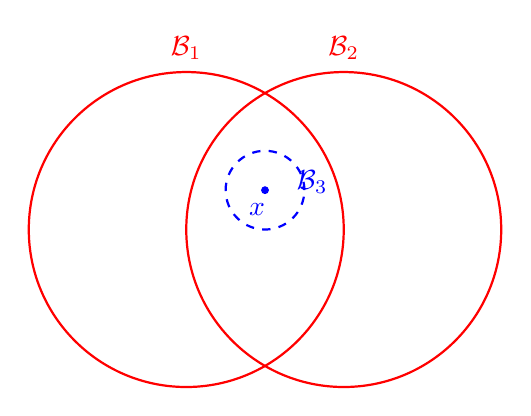
\begin{tikzpicture}[scale=1]
    
      % Ball B1
      \draw[red, thick] (0,0) circle (2);
      \node[red] at (0,2.3) {$\mathcal{B}_1$};
    
      % Ball B2
      \draw[red, thick] (2,0) circle (2);
      \node[red] at (2,2.3) {$\mathcal{B}_2$};
    
      % Point x and its neighborhood B3
      \filldraw[blue] (1,0.5) circle (1.2pt); % point x
      \node[blue] at (0.9,0.25) {$x$};
      \draw[blue, dashed, thick] (1,0.5) circle (0.5);
      \node[blue] at (1.6,0.6) {$\mathcal{B}_3$};
    \end{tikzpicture}
    
\end{center}

\paragraph{Demostración.}
Definimos una familia $\mathcal T_{\mathcal B}$ de subconjuntos de $X$:
\[
  \mathcal T_{\mathcal{B}}
  = \bigl\{\,U\subseteq X : U = \bigcup \mathcal{B}',\ \mathcal{B}'\subseteq\mathcal{B}\bigr\}.
\]
Hay que mostrar que $\mathcal T_{\mathcal{B}}$ es una topología en $X$. Para ello, probamos las cuatro propiedades:

\begin{enumerate}[label=\arabic*.]
  \item $\emptyset \in  \mathcal T_{\mathcal{B}}$, pues sea $\emptyset \subseteq \mathcal{B}$, la subfamilia vacía entonces:
    \begin{align*}
      \emptyset &= \bigcup \emptyset,
    \end{align*}

  \item $X\in\mathcal T_{\mathcal{B}}$, para esto veamos que:
    \begin{align*}
      X &= \bigcup \mathcal{B},
    \end{align*}
    es decir que:
    \begin{enumerate}[label=\alph*)]
        \item[$\supseteq$] Por la parte 1 de la definición de base, si $x\in X$ existe $B\in\mathcal{B}$ tal que $x\in B$ y por lo tanto $x\in \bigcup \mathcal{B}$.
        \item[$\subseteq$] Si $x\in \bigcup \mathcal{B}$, entonces existe $B\in\mathcal{B}$ tal que $x\in B$, pero $B\subseteq X$, por lo que $x\in X$. Asi que $X\subseteq \bigcup \mathcal{B}$.
    \end{enumerate}
    Por lo tanto $X=\bigcup \mathcal{B}$.

  \item \textbf{Uniones arbitrarias:} Sea $\{U_i\}_{i\in I}\subseteq \mathcal T_{\mathcal{B}}$. Por la definicion de $\mathcal T_{\mathcal B}$ se tiene que para cada $i$, existe $\mathcal{B}_i\subseteq\mathcal{B}$ tal que
    \[
      U_i = \bigcup \mathcal{B}_i.
    \]

    Entonces
    \begin{align*}
      \bigcup_{i\in I} U_i
      &= \bigcup_{i\in I}\Bigl(\bigcup \mathcal{B}_i\Bigr)
      = \bigcup\Bigl(\bigcup_{i\in I}\mathcal{B}_i\Bigr)
      = \bigcup \mathcal{B}', 
    \end{align*}
    donde $\mathcal{B}'=\bigcup_{i\in I}\mathcal{B}_i\subseteq\mathcal{B}$. Así, $\bigcup_{i\in I}U_i\in\mathcal T_{\mathcal{B}}$.

  \item \textbf{Intersecciones finitas:} Sea $U_1,\dots,U_n\in\mathcal T_{\mathcal{B}}$. Para cada $k=1,\dots, n$, existe $\mathcal{B}_k\subseteq\mathcal{B}$ tal que
    \[
      U_k = \bigcup \mathcal{B}_k.
    \]
    Procedemos por inducción en $n$. Para $n=2$:
    \[
      U_1\cap U_2
      = \Bigl(\bigcup \mathcal{B}_1\Bigr)\cap \Bigl(\bigcup \mathcal{B}_2\Bigr).
    \]
    Hay dos casos:
    \begin{itemize}
      \item Caso 1: $U_1\cap U_2=\emptyset$. Entonces $\emptyset\in\mathcal T_{\mathcal{B}}$.
      \item Caso 2: $U_1\cap U_2\neq\emptyset$. Sea $x\in U_1\cap U_2$. Entonces existen $B_1\in\mathcal{B}_1$ y $B_2\in\mathcal{B}_2$ con $x\in B_1\cap B_2$. Por la condición de base, existe $B_3\in\mathcal{B}$ tal que
      \[
        x\in B_3\subseteq B_1\cap B_2.
      \]
      Sea 
      \[
        \mathcal{B}_3 = \{\,B\in\mathcal{B} : B\subseteq U_1\cap U_2\}.
      \]
      Entonces
      \begin{align*}
        \bigcup \mathcal{B}_3 = U_1\cap U_2,
      \end{align*}
      \begin{itemize}
        \item[$\supseteq$] Si $x \in \mathcal {B}_3$, entonces $x\in B_3\subseteq B_1\cap B_2$ y por lo tanto $x\in U_1\cap U_2$.
        \item[$\subseteq$] Si $x\in U_1\cap U_2$, entonces existen $B_1\in\mathcal{B}_1$ y $B_2\in\mathcal{B}_2$ tales que $x\in B_1\cap B_2$. Por la condición de base, existe $B_3\in\mathcal{B}$ tal que $x\in B_3\subseteq B_1\cap B_2$. Por lo tanto $x\in \mathcal{B}_3$.
      \end{itemize}
    \end{itemize}
    El paso inductivo para $n>2$ se realiza de manera análoga.
\end{enumerate}

Por tanto, $\mathcal T_{\mathcal{B}}$ es una topología en $X$.